% move all configuration stuff into one file so we can focus on the content
\documentclass[aspectratio=169,hyperref={pdfpagelabels=false,colorlinks=true,linkcolor=white,urlcolor=blue},t]{beamer}

%%%%%%%%%%%%%%%%%%%%%%%%%%%%%%%%%%%%%%%%%%%%%%%%%%%%%%%%%%%%%%%%%%%%%%%%%%%%%%%%%%
%%%%%%%%%%%%%%%%%%%%%%%%%%%%%%%%%%%%%%%%%%%%%%%%%%%%%%%%%%%%%%%%%%%%%%%%%%%%%%%%%%
% packages
\usepackage{pict2e}
\usepackage{epic}
\usepackage{amsmath,amsfonts,amssymb}
\usepackage{units}
\usepackage{fancybox}
\usepackage[absolute,overlay]{textpos} 
\usepackage{media9} % avi2flv: "C:\Program Files\ffmpeg\bin\ffmpeg.exe" -i TuneFreqFilterbank.avi -b 600k -s 441x324 -r 15 -acodec copy TuneFreqFilterbank.flv
\usepackage{animate}
\usepackage{gensymb}
\usepackage{multirow}
\usepackage{silence}
\usepackage[backend=bibtex,style=ieee]{biblatex}
\AtEveryCitekey{\iffootnote{\tiny}{}}
\addbibresource{references}

%%%%%%%%%%%%%%%%%%%%%%%%%%%%%%%%%%%%%%%%%%%%%%%%%%%%%%%%%%%%%%%%%%%%%%%%%%%%%%%%%%
%%%%%%%%%%%%%%%%%%%%%%%%%%%%%%%%%%%%%%%%%%%%%%%%%%%%%%%%%%%%%%%%%%%%%%%%%%%%%%%%%%
% relative paths
\graphicspath{{graph/}}


%%%%%%%%%%%%%%%%%%%%%%%%%%%%%%%%%%%%%%%%%%%%%%%%%%%%%%%%%%%%%%%%%%%%%%%%%%%%%%%%%%
%%%%%%%%%%%%%%%%%%%%%%%%%%%%%%%%%%%%%%%%%%%%%%%%%%%%%%%%%%%%%%%%%%%%%%%%%%%%%%%%%%
% units
\setlength{\unitlength}{1mm}

%%%%%%%%%%%%%%%%%%%%%%%%%%%%%%%%%%%%%%%%%%%%%%%%%%%%%%%%%%%%%%%%%%%%%%%%%%%%%%%%%%
%%%%%%%%%%%%%%%%%%%%%%%%%%%%%%%%%%%%%%%%%%%%%%%%%%%%%%%%%%%%%%%%%%%%%%%%%%%%%%%%%%
% theme & layout
\usetheme{Frankfurt}
\beamertemplatenavigationsymbolsempty
%\setbeamertemplate{frametitle}[smoothbars theme]
\setbeamertemplate{frametitle}
{
    \begin{beamercolorbox}[ht=1.8em,wd=\paperwidth]{frametitle}
        \vspace{-.1em}%
        \hspace{.2em}{\strut\insertframetitle\strut}
        
        \hspace{.2em}\small\strut\insertframesubtitle\strut
        %\hfill
        %
\includegraphics[height=.8cm,keepaspectratio]{CenterMusicTechnology-solid-2lines-white-CoAtag}
        
    \end{beamercolorbox}
    \begin{textblock*}{100mm}(11.6cm,.7cm)
        \includegraphics[height=.8cm,keepaspectratio]{logo_GTCMT_black}
    \end{textblock*}
}

% set this to ensure bulletpoints without subsections
\usepackage{remreset}
\makeatletter
\@removefromreset{subsection}{section}
\makeatother
\setcounter{subsection}{1}

%---------------------------------------------------------------------------------
% appearance
\setbeamercolor{structure}{fg=gtgold}
\setbeamercovered{transparent} %invisible
\setbeamercolor{bibliography entry author}{fg=black}
\setbeamercolor*{bibliography entry title}{fg=black}
\setbeamercolor*{bibliography entry note}{fg=black}

%\usepackage{pgfpages}
%\setbeameroption{show notes}
%\setbeameroption{show notes on second screen=right}
%---------------------------------------------------------------------------------
% fontsize
\let\Tiny=\tiny

%%%%%%%%%%%%%%%%%%%%%%%%%%%%%%%%%%%%%%%%%%%%%%%%%%%%%%%%%%%%%%%%%%%%%%%%%%%%%%%%%%
%%%%%%%%%%%%%%%%%%%%%%%%%%%%%%%%%%%%%%%%%%%%%%%%%%%%%%%%%%%%%%%%%%%%%%%%%%%%%%%%%%
% warnings
\pdfsuppresswarningpagegroup=1
\WarningFilter{biblatex}{Patching footnotes failed}
\WarningFilter{latexfont}{Font shape}
\WarningFilter{latexfont}{Some font shapes}
\WarningFilter{gensymb}{Not defining}



\newcommand{\listspectralfeature}[2]{
\vspace{-5mm}
\begin{equation*}
    \input{eq/Spectral#1}
\end{equation*}
\only<2>{
    \question{discuss the feature}
    \begin{itemize}
        \item   how would you describe its 'meaning'
        \item   value of this feature for the hypothetical prototype signals
            \begin{itemize}
                \item   silence
                \item   single peak (@ $k_\mathrm{s}$)
                \item   white noise (flat magnitude spectrum)
            \end{itemize}
    \end{itemize}
}
\only<3>{
    \vspace{-3mm}
    \figwithref{FeaturesSpectral#1}{matlab source: matlab/displayFeatures.m}
}
\only<4>{
    %\vspace{10mm}
    
    \textbf{common variants}:
    
    #2
    }
\vspace{50mm}
}                    


\subtitle{Part 4.2: Instantaneous Features~---~Spectral Shape}

%%%%%%%%%%%%%%%%%%%%%%%%%%%%%%%%%%%%%%%%%%%%%%%%%%%%%%%%%%%%%%%%%%%%%%%%%%%%
\begin{document}
    % generate title page
	

\begin{frame}
    \titlepage
    %\vspace{-5mm}
    \begin{flushright}
        \href{http://www.gtcmt.gatech.edu}{\includegraphics[height=.8cm,keepaspectratio]{logo_GTCMT_black}}
    \end{flushright}
\end{frame}


    \section[overview]{lecture overview}
        \begin{frame}{instantaneous features}{overview}
            \begin{itemize}
                \item   \textbf{text book}  
                    \begin{itemize}
                        \item   \href{http://ieeexplore.ieee.org/xpl/ebooks/bookPdfWithBanner.jsp?fileName=6331120.pdf&bkn=6266785&pdfType=chapter}{\underline{\textit{Chapter 3: Instantaneous Features} (pp.~41--63)}}
                    \end{itemize}
                \bigskip
                \item<2->   \textbf{lecture content}
                    \begin{itemize}
                        \item<2->   spectral shape and timbre
                        \item<3->   spectral features
                        \item<4->   features of general signal properties
                    \end{itemize}
            \end{itemize}
        \end{frame}

    \section[intro]{introduction}
        \begin{frame}{instantaneous features}{introduction}
            remember the flow chart of a general ACA system:
            \vspace{-2mm}
            \begin{figure}
                \begin{footnotesize}
				\begin{picture}(96,26)
					\setcounter{iXOffset}{0}
					\setcounter{iYOffset}{5}
					\setcounter{iXBlockSize}{28}
					\setcounter{iYBlockSize}{16}
					\setcounter{iYBlockSizeDiv2}{8}
					\setcounter{iDistance}{8}
	
					\addtocounter{iYOffset}{\value{iYBlockSizeDiv2}}
					\addtocounter{iYOffset}{-2}
	
					%\addtocounter{iXOffset}{-1}
					\put(\value{iXOffset}, \value{iYOffset})
						{\text{{\shortstack[c]{audio\\ signal}}}}
					\addtocounter{iXOffset}{1}
	
					\addtocounter{iYOffset}{2}
					\addtocounter{iXOffset}{\value{iDistance}}
	
					\put(\value{iXOffset}, \value{iYOffset})
						{\vector(1,0){\value{iDistance}}}
	
					\addtocounter{iXOffset}{\value{iDistance}}
					\addtocounter{iYOffset}{-\value{iYBlockSizeDiv2}}
					
					\put(\value{iXOffset}, \value{iYOffset})
						{\framebox(\value{iXBlockSize}, \value{iYBlockSize}) {\color{gtgold}{\shortstack[c]{feature\\ extraction}}}}
	
					\addtocounter{iXOffset}{\value{iXBlockSize}}
					\addtocounter{iYOffset}{\value{iYBlockSizeDiv2}}
	
					\put(\value{iXOffset}, \value{iYOffset})
						{\vector(1,0){\value{iDistance}}}
	
					\addtocounter{iXOffset}{\value{iDistance}}
					\addtocounter{iYOffset}{-\value{iYBlockSizeDiv2}}
	
					\put(\value{iXOffset}, \value{iYOffset})
						{\framebox(\value{iXBlockSize}, \value{iYBlockSize}) {\shortstack[c]{decision,\\ interpretation,\\ classification,\\ inference}}}
	
					\addtocounter{iXOffset}{\value{iXBlockSize}}
					\addtocounter{iYOffset}{\value{iYBlockSizeDiv2}}
	
					\put(\value{iXOffset}, \value{iYOffset})
						{\vector(1,0){\value{iDistance}}}
	
					\addtocounter{iXOffset}{\value{iDistance}}
					\addtocounter{iYOffset}{-2}
	
					\addtocounter{iXOffset}{1}
					\put(\value{iXOffset}, \value{iYOffset})
						{\text{{\shortstack[c]{meta\\ data}}}}
					
				\end{picture}
\end{footnotesize}

            \end{figure}
        \end{frame}
        
        \begin{frame}{instantaneous features}{introduction~---~timbre 1/2}
            \begin{block}{\textbf{definition (American Standards Association)}}
                ...that attribute of sensation in terms of which a listener can judge that two sounds having the same loudness and pitch are dissimilar
            \end{block}
            \pause
            \question{What is the problem with this definition?}
            \vspace{-5mm}
            Bregman:\footfullcite{bregman_auditory_1994}
                    \begin{enumerate}
                        \item   implies that timbre \textit{only} exists for sound with pitch!
                        \item   only says that timbre \textit{is not} loudness and pitch
                    \end{enumerate}
            \pause
            
            \begin{itemize}
                \item[$\rightarrow$]   [timbre is] "\textit{...the psychoacoustician's multidimensional waste-basket category for everything that cannot be labeled pitch or loudness.}"\footfullcite{mcadams_hearing_1979}
            \end{itemize}
        \end{frame}
        
        \begin{frame}{instantaneous features}{introduction~---~timbre 2/2}
        
            timbre is
            \begin{itemize}
                \item   a function of \textbf{temporal envelope}
                    \begin{itemize}
                        \item   attack time characteristics
                        \item   amplitude modulations
                        \item   \ldots
                    \end{itemize}
                \item<2->   a function of \color<3->{gtgold}{\textbf{spectral distribution}}
                    \begin{itemize}
                        \item   spectral envelope
                        \item   number of partials
                        \item   energy distribution of partials
                        \item   \ldots
                    \end{itemize}
            \end{itemize}

            \begin{itemize}
                \item<3->[] when dealing with complex mixtures of sound, it is very difficult (maybe impossible?) to extract detailed temporal information for individual tones
                \item<4->[$\Rightarrow$] features typically focus on the \textbf{spectral shape}
            \end{itemize}
        \end{frame}

    \section[spectral shape]{spectral features}
        \begin{frame}{instantaneous features}{timbre: spectral rolloff}
            \listspectralfeature{Rolloff}{\begin{itemize}   \item restricted frequency range  \item power spectrum  \end{itemize}}
        \end{frame}
        \begin{frame}{instantaneous features}{timbre: spectral flux}
            \listspectralfeature{Flux}{\begin{itemize} \item different distance measure
						\begin{footnotesize}
							\item[]
							\begin{eqnarray*}
								v_{\mathrm{SF}}(n, \beta) &=& \frac{\sqrt[\beta]{\sum\limits_{k = 0}^{\mathcal{K}/2-1}{\left(|X(k,n)|-|X(k,n-1)|\right)^\beta}}}{\nicefrac{\mathcal{K}}{2}}\\
								v_{\mathrm{SF}, \sigma}(n) &=& \sqrt{{\frac{2}{\mathcal{K}}}\sum\limits_{k = 0}^{\mathcal{K}/2-1}{\left(\Delta X(k,n)-\mu_{\Delta X}\right)^2}}\\
								v_\mathrm{SF, log}(n) &=& {{\frac{2}{\mathcal{K}}}\sum\limits_{k = 0}^{\mathcal{K}/2-1}{\log_2\left(\frac{|X(k,n)|}{|X(k,n-1)|}\right)}}
							\end{eqnarray*}
						\end{footnotesize}\end{itemize}}
        \end{frame}
        \begin{frame}{instantaneous features}{timbre: spectral centroid}
            \listspectralfeature{Centroid}{\begin{itemize}  \item magnitude spectrum vs.\ power spectrum    \item logarithmic frequency scale
						\[
							v_\mathrm{SC,log}(n) = \frac{\sum\limits_{k = k(f_{\mathrm{min}})}^{\mathcal{K}/2-1}{\log_2\left(\frac{f(k)}{f_{\mathrm{ref}}}\right)\cdot |X(k,n)|^2}}{\sum\limits_{k = k(f_{\mathrm{min}})}^{N/2-1}{|X(k,n)|^2}} 
						\]
			\end{itemize}}
        \end{frame}
        \begin{frame}{instantaneous features}{timbre: spectral spread}
            \listspectralfeature{Spread}{\begin{itemize}    \item same variants as with \textit{spectral Centroid}, e.g.\ logarithmic:
				\begin{footnotesize}\[
                        v_\mathrm{SS,log}(n) = \sqrt{\frac{\sum\limits_{k = k(f_{\mathrm{min}})}^{\nicefrac{\mathcal{K}}{2}-1}{\left(\log_2\left(\frac{f(k)}{\unit[1000]{Hz}}\right)-v_{\mathrm{SC}}(n)\right)^2\cdot |X(k,n)|^2}}{\sum\limits_{k = k(f_{\mathrm{min}})}^{\nicefrac{\mathcal{K}}{2}-1}{|X(k,n)|^2}}} 
                    \]\end{footnotesize}
			\end{itemize}}
        \end{frame}
        \begin{frame}{instantaneous features}{timbre: spectral decrease}
            \listspectralfeature{Decrease}{\begin{itemize}  \item restricted frequency range:
					\[
						v_{\mathrm{SD}}(n) = \frac{\sum\limits_{k = k_{\mathrm{l}}}^{k_{\mathrm{u}}}\frac{1}{k}\cdot \big(|X(k,n)|-|X(k_{\mathrm{l}}-1,n)|\big)}{\sum\limits_{k = k_{\mathrm{l}}}^{k_{\mathrm{u}}}{|X(k,n)|}} 
					\]  \end{itemize}}
        \end{frame}
        \begin{frame}{instantaneous features}{timbre: spectral slope}
            \listspectralfeature{Slope}{}
        \end{frame}
        \begin{frame}{instantaneous features}{timbre: spectral skewness}
            \listspectralfeature{Skewness}{}
        \end{frame}
        \begin{frame}{instantaneous features}{timbre: spectral kurtosis}
            \listspectralfeature{Kurtosis}{}
        \end{frame}

		\begin{frame}{fundamentals}{cepstrum 1/3}
			\textbf{signal model}: \\
			convolution of \textit{excitation signal} and \textit{transfer function}
			\begin{equation*}\label{eq:speech}
				x(i) = e(i)\ast h(i)
			\end{equation*}
			\pause
			\begin{equation*}
				X(\jom) = E(\jom)\cdot H(\jom) 
			\end{equation*}
			\pause
			\begin{eqnarray*}
				\log\big(X(\jom)\big)	&=& \log\big(E(\jom)\cdot H(\jom)\big)\nonumber\\
											&=& \log\big(E(\jom)\big) \mathbf{+} \log\big(H(\jom)\big) 
			\end{eqnarray*}
		\end{frame}

		\begin{frame}{fundamentals}{cepstrum 2/3}
			\vspace{-4mm}
            \begin{eqnarray*}
				c_x(i)	&=& \mathfrak{F}^{-1}\left\{\log\left(X(\jom)\right)\right\}\nonumber\\
                        \pause
						&=& \mathfrak{F}^{-1}\left\{\log\left(E(\jom)\right) + \log\left(H(\jom)\right)\right\}\nonumber\\
						\pause
                        &=& \mathfrak{F}^{-1}\left\{\log\left(E(\jom)\right)\right\} + \mathfrak{F}^{-1}\left\{\log\left(H(\jom)\right)\right\} \\
                    \pause
					\hat{c}_x(i_{\mathrm{s}}(n)\ldots i_{\mathrm{e}}(n)) &=& \sum\limits_{k=0}^{\nicefrac{\mathcal{K}}{2}-1}{\log\left(|X(k,n)|\right)\e^{\mathrm{j}ki\Delta\Omega}} 
			\end{eqnarray*}
				
			\vspace{-4mm}
            \figwithmatlab{Cepstrum}
		\end{frame}
        
        \begin{frame}{fundamentals}{cepstrum 3/3}
            \begin{itemize}
                \item \textbf{summary}:
                    \begin{itemize}
                        \item   cepstrum replaces the convolution operation with addition
                        \item   result is the \textit{unfiltered} excitation signal plus the filter IR (both logarithmic)
                        \item   can be used for, e.g., \textit{spectral envelope extraction} or \textit{pitch detection}
                        \item<2> the naming silliness knows no boundaries:\\
                         cepstrum, quefrequency, liftering, \ldots
                    \end{itemize}
            \end{itemize}
        \end{frame}

		\begin{frame}{instantaneous features}{timbre: mel frequency cepstral coefficients 1/4}
            \begin{itemize}
                \item   typical processing steps for the mel frequency cepstral coefficients (MFCCs):
                    \begin{enumerate}
                        \item   compute magnitude spectrum
                        \item   convert linear frequency scale to logarithmic
                        \item   group bins into bands
                        \item   apply logarithm to all bands
                        \item   compute (inverse) cosine transform (DCT)
                    \end{enumerate}
            \end{itemize}
            
            \bigskip
			\begin{equation*}
				v^j_{\mathrm{MFCC}}(n)	= \sum\limits_{k' = 1}^{\mathcal{K}'}{\log\big( |X'(k',n)|\big)\cdot \cos\left( j\cdot\left(k'-\frac{1}{2} \right)\frac{\pi}{\mathcal{K}'} \right)}			
			\end{equation*}
        \end{frame}

		\begin{frame}{instantaneous features}{timbre: mel frequency cepstral coefficients 2/4}
			\figwithmatlab{MfccFilterbank}
            
            \begin{itemize}
                \item   constant Q filter spacing for higher frequencies (mel scale)
                \item   FFT values are weighted and summed over bins for each band
            \end{itemize}
		\end{frame}
		\begin{frame}{instantaneous features}{timbre: mel frequency cepstral coefficients 3/4}
			\begin{columns}
                \column{.75\textwidth}
                    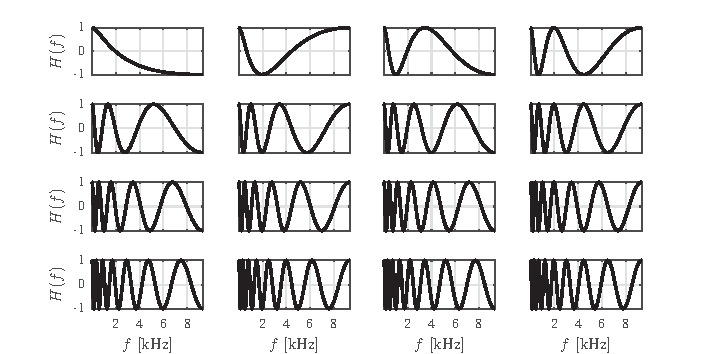
\includegraphics[scale=.4]{MfccMelDct}
                \column{.25\textwidth}
                    mel-warped cosine functions for DCT
			\end{columns}
		\end{frame}
		\begin{frame}{instantaneous features}{timbre: mel frequency cepstral coefficients 4/4}
			\vspace{-5mm}\begin{footnotesize}
			\begin{table}
				\centering
				\begin{tabular*}{\textwidth}{@{\extracolsep{\fill}}lccc}%{l|c|c|c} %{c|p{12mm}p{12mm}p{12mm}p{12mm}p{12mm}p{12mm}p{12mm}}
                    \\ \hline
                    \bf{\emph{Property}}	 & \bf{\emph{DM}}	 & \bf{\emph{HTK}}	 & \bf{\emph{SAT}}\\ 
                     \hline
                    \bf{Num.\ filters}	 & 20	 & 24	 & 40\\
                    \bf{Mel scale}	 & lin/log	 & log	 & lin/log\\
                    \bf{Freq.\ range}	 & $[100; 4000]$	 & $[100; 4000]$	 & $[200; 6400]$\\
                    \bf{Normalization}	 & Equal height	 & Equal height	 & Equal area\\
				\end{tabular*}
			\end{table}
			\end{footnotesize}

            \vspace{-5mm}
            \figwithref{FeaturesSpectralMfccs}{matlab source: matlab/displayFeatures.m}
		\end{frame}

    \section[tonalness]{tonalness features}
        \begin{frame}{instantaneous features}{tonalness: spectral crest factor}
            \listspectralfeature{CrestFactor}{\begin{itemize}   \item normalization \item power spectrum \item measure \textit{per band} instead of  whole spectrum \end{itemize}}
        \end{frame}
        \begin{frame}{instantaneous features}{tonalness: spectral flatness}
            \listspectralfeature{Flatness}{\begin{itemize}   \item power vs.\ magnitude spectrum \item smoothed spectrum (avoid spurious 0-bins) \item measure \textit{per band} instead of  whole spectrum \end{itemize}}
        \end{frame}
        \begin{frame}{instantaneous features}{tonalness: spectral tonal power ratio}
            \listspectralfeature{TonalPowerRatio}{\begin{itemize}   \item definition of tonal/non-tonal components \end{itemize}}
        \end{frame}
        
		\begin{frame}{instantaneous features}{tonalness: maximum of ACF 1/2}
			\begin{equation*}
				v_{\mathrm{Ta}}(n)	= \max\limits_{0\leq \eta \leq \mathcal{K}-1}{|r_{xx}(\eta,n)|}
			\end{equation*}
            \only<2>{
                \question{discuss the feature}
                \begin{itemize}
                    \item   how would you describe its 'meaning'
                    \item   value of this feature for the hypothetical prototype signals
                        \begin{itemize}
                            \item   silence
                            \item   periodic signal ($T_0 = k$)
                            \item   white noise (flat magnitude spectrum)
                        \end{itemize}
                \end{itemize}
            }
            \only<3>{
                \vspace{-3mm}
                \figwithref{FeaturesTimeMaxAcf}{matlab source: matlab/displayFeatures.m}
            }
		\end{frame}
		\begin{frame}{instantaneous features}{tonalness: maximum of ACF 2/2}
            \question{maximumdetection: how to avoid main lobe maxima?}
			
			\begin{itemize}
				\item	minimum lag
				\item	magnitude threshold
				\item	search only after first local minimum
			\end{itemize}
		\end{frame}
        %Predictivity Ratio
        %SpectralPredictivity

    \section[technical]{technical properties}
		\begin{frame}\frametitle{signal properties}\framesubtitle{zero crossing rate}
			\begin{equation*}\label{eq:zc}
				v_{\mathrm{ZC}}(n) = \frac{1}{2 \cdot\mathcal{K}}\sum\limits_{i=i_{\mathrm{s}}(n)}^{i_{\mathrm{e}}(n)}{\big|\sign \left[x(i)\right]-\sign \left[x(i-1)\right]\big|} 
			\end{equation*}
            \only<2>{
                \question{discuss the feature}
                \begin{itemize}
                    \item   how would you describe its 'meaning'
                    \item   value of this feature for the hypothetical prototype signals
                        \begin{itemize}
                            \item   silence
                            \item   periodic signal ($T_0 = k$)
                            \item   white noise (flat magnitude spectrum)
                        \end{itemize}
                \end{itemize}
            }
            \only<3>{
                \vspace{-3mm}
                \figwithref{FeaturesTimeZeroCrossingRate}{matlab source: matlab/displayFeatures.m}
            }
		\end{frame}
		\begin{frame}\frametitle{signal properties}\framesubtitle{ACF coefficients}
			\begin{equation*}
				v^{\eta}_{\mathrm{ACF}}(n)	= r_{xx}(\eta,n) \quad \text{with}\enspace \eta = 1,2,3,\ldots
			\end{equation*}
            \only<2>{
                \question{discuss the feature}
                \begin{itemize}
                    \item   how would you describe its 'meaning'
                    \item   value of this feature for the hypothetical prototype signals
                        \begin{itemize}
                            \item   silence
                            \item   periodic signal ($T_0 = k$)
                            \item   white noise (flat magnitude spectrum)
                        \end{itemize}
                \end{itemize}
            }
            \only<3>{
                \vspace{-3mm}
                \figwithref{FeaturesTimeAcfCoeff}{matlab source: matlab/displayFeatures.m}
            }
		\end{frame}

    \section[learned]{feature learning}
        \begin{frame}{instantaneous features}{feature learning}
            \textbf{TODO: SLIDES UNFINISHED}
            \begin{itemize}
                \item   low-level features are relatively simple to compute, and possibly have only limited meaningfulness
                \item   alternative: try to learn features from the data (usually unsupervised)
                \item   \textbf{principle}
                    \begin{itemize}
                        \item   put (a lot of) raw data at input, learn a way of reducing dimensionality
                    \end{itemize}
                \item   \textbf{advantages}
                    \begin{itemize}
                        \item   features might contain more useful information than provided by hand-crafted features
                        \item   no expert knowledge needed
                        \item   possibly easier generalization
                    \end{itemize}
                \item   \textbf{disadvantages}
                    \begin{itemize}
                        \item   usually time consuming
                        \item   limited ways of controlling the type of information learned
                    \end{itemize}
            \end{itemize}
            \bigskip
            \begin{itemize}
                \item   dictionary learning (sparse coding, nmf)
                \item   neural networks and deep architectures (also semi-supervised and supervised)
                \item   clustering (distance/similarity of point to cluster)
                \item   PCA etc
            \end{itemize}
        \end{frame}

    \section[summary]{lecture summary}
        \begin{frame}{summary}{lecture content}
            \begin{enumerate}
                \item   how do you describe and characterize timbre in music
                \smallskip
                \item<2->   name 5 low level features
                \smallskip
                \item<3->   what would be typical algorithm parameters to extract, e.g., the \textit{spectral centroid}
            \end{enumerate}
        \end{frame}
\end{document}

